\documentclass[11pt]{article}

\usepackage[margin=1in, headheight=14.5pt]{geometry}
\usepackage{amsfonts, amsmath, amssymb}
\usepackage[none]{hyphenat}
\usepackage{fancyhdr}
\usepackage[spanish]{babel}
\usepackage[spanish, calc]{datetime2}
\usepackage{fmtcount}
\usepackage{graphicx}
\usepackage{float}
\usepackage[nottoc, notlot, notlof]{tocbibind}
\usepackage{tocloft}
\usepackage[utf8]{inputenc}
\usepackage{parskip}
\usepackage{xcolor}
\usepackage{cancel}
\usepackage{textcomp}
\usepackage{pgfplots}
\usepackage{tikz}
\usetikzlibrary{datavisualization}
\usetikzlibrary{datavisualization.formats.functions}
\pgfplotsset{compat=1.15}
\usepackage{mathrsfs}
\usetikzlibrary{arrows}

\parindent 0ex

\pgfplotsset{width=10cm,compat=1.9}

\def\imj{\mathrm{j}}
\def\sen{\mathrm{sen}}

\renewcommand\cftsecleader{\cftdotfill{\cftdotsep}}
\renewcommand{\baselinestretch}{1.1}
\newcommand*\circled[1]{\tikz[baseline=(char.base)]{
		\node[shape=circle,draw,inner sep=2pt] (char) {#1};}}

\graphicspath{{C:/Users/tomas/OneDrive/Escritorio/LATEX/matematica-superior/commons/img/}}

\pagestyle{fancy}
\fancyhead{}
\fancyfoot{}
\fancyhead[L]{\MakeUppercase{Matemática Superior}}
\fancyhead[R]{\slshape Serie de Fourier: Ejercicios de final}
\fancyfoot[C]{\thepage}


\begin{document}
		
	\begin{titlepage}
		\begin{center}
			\vspace*{0.5cm}
			\Large{\textbf{Universidad Tecnológica Nacional}}\\
			\Large{\textbf{Facultad Regional Buenos Aires}}\\
			\begin{center}
				
\includegraphics[scale=0.4]{logoutn.png}
			\end{center}
			\vfill
			\line(1,0){400}\\
			\vspace*{0.3cm}
			\huge{\textbf{Matemática Superior}}\\
			\Large{\textbf{Unidad 2: Series y Transformadas de Fourier}}\\
			\large{Ejercicios resueltos de final}
			\line(1,0){400}\\
			\vfill
			Tomás Moreira \\
			
			\DTMnewdatestyle{mydate}{%
				\renewcommand{\DTMdisplaydate}[4]{%
					\DTMMonthname{##2} \number##1
				}
				\renewcommand{\DTMDisplaydate}{\DTMdisplaydate}
			}
			
			\DTMsetdatestyle{mydate}
			\today
				
				
		\end{center}
	\end{titlepage}

	\tableofcontents
	\thispagestyle{empty}
	\clearpage

	\setcounter{page}{1}
	\section{Introducción}
	Esta recopilación está tomada de algunos finales que están disponibles en el aula virtual general de la materia, y algunos son de finales más nuevos (2018-2020). Las soluciones aquí planteadas cuentan con un mayor nivel de detalle.
	\section{Ejercicio 1}
	Final 19/12/2017. \textit{Elegir la respuesta correcta}:\\
	Dada la función $f(x)=e^{x}-1$ en $\left[0,1\right)$, para que tenga simetría de media onda con período $T=2$ hay que definirla en $\left[1,2\right)$:
	\renewcommand{\labelenumi}{\alph{enumi})}
	\begin{enumerate}
		\item $f(x)=-e^{x}+1$
		\item $f(x)=-e^{x-1}+1$
		\item $f(x)=-e^{x-1}-1$
		\item Ninguna de las anteriores.
	\end{enumerate}

	\textbf{Resolución:}
	
	Empecemos graficando nuestra función:\\
	\begin{center}
		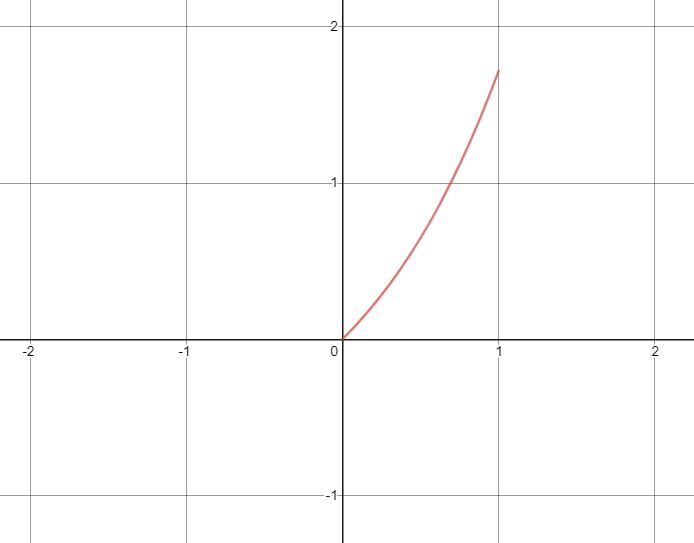
\includegraphics[scale=0.6]{02-SerieYTransformadaDeFourier/final1_1.JPG}
	\end{center}

	Podemos realizar el ejercicio en forma gráfica. Para ello, como sabemos que nuestro período de la nueva función será $T=2$, tenemos que desplazar nuestra función medio período (es decir, graficarla en el $(1,2)$) y luego espejarla con respecto al eje de abscisas, de la siguiente manera:\\
	
	\begin{center}
		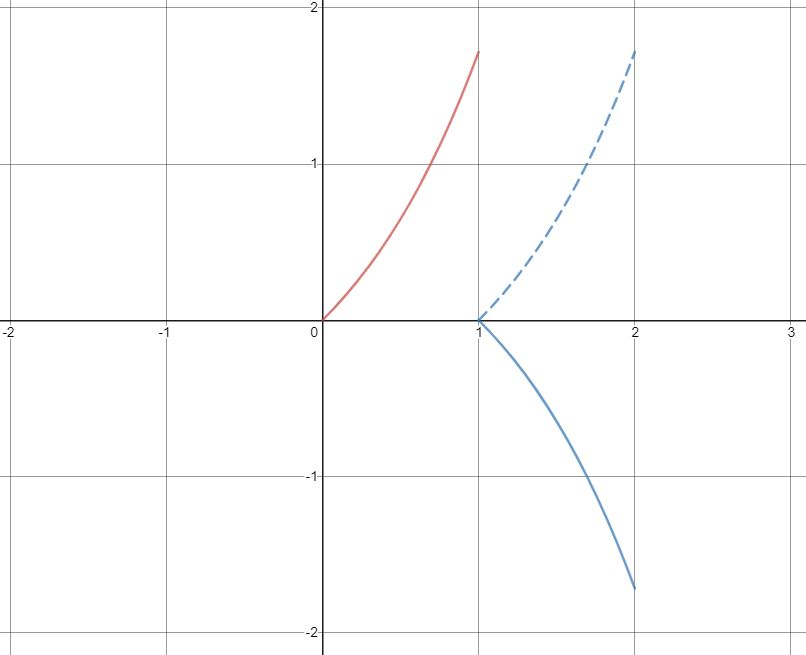
\includegraphics[scale=0.6]{02-SerieYTransformadaDeFourier/final1_2.JPG}
	\end{center}

	Luego, sería cuestión de deducir la forma de la función.
	
	En forma analítica, podemos usar la definición de función con simetría de media onda:	
	$$f(x)=-f(x+L)$$ Donde $L$ es el semiperiodo, es decir $T/2$.
	
	En nuestro caso sabemos que $T=2$, por ende $L=1$, aunque como el otro trozo de función lo piden en un desplazamiento hacia la derecha, vamos a tomarnos el atrevimiento de usar $f(x)=-f(x-L)$. En nuestro caso, $f(x)=-f(x-1)$
	
	Reemplazamos: $f(x)=-\left(e^{(x-1)}-1\right)$
	
	Distribuimos y sacamos los paréntesis redundantes, llegando a la función en forma analítica:\\
	$\boxed{f(x)=-e^{x-1}+1}$
	
	Por lo tanto, la respuesta correcta es la \fcolorbox{black}{yellow}{\circled{b}}.
	\section{Ejercicio 2}
	Final 22/02/2018. \textit{Indicar verdadero o falso}:\\
	La función $   
	f(x) = 
	\begin{cases}
	5 &\quad\text{si}\;-2\leq x \leq 2\\
	2 &\quad\text{si}\;\;2< |x| < 3 \\
	\end{cases}
	\enspace\wedge\enspace
	f(x)=f(x+6)
	$
	tiene valor medio $4$.
	\section{Ejercicio 3}
	Final 15/02/2018. \textit{Indicar verdadero o falso}:\\
	Al desarrollar la función $f(t)=\sen\left(\pi t\right)$ si $t\in(0,1) \wedge f(t)=f(t+1)$ en Serie Exponencial de Fourier sólo hay términos con coeficientes reales.
	\section{Ejercicio 4}
	Final 12/12/2017. \textit{Indicar la respuesta correcta}:\\
	La Serie Exponencial de Fourier de $f(x)=4-x$ si $x\in(0,2) \wedge f(x)=f(x+2)$ tiene los coeficientes:
	\renewcommand{\labelenumi}{\alph{enumi})}
	\begin{enumerate}
		\item Todos reales.
		\item Todos imaginarios.
		\item Uno real y resto imaginarios.
		\item Ninguna de los anteriores.
	\end{enumerate}
	\section{Ejercicio 5}
	Final 07/10/2016. \textit{Desarrollar}:\\
	El desarrollo de $f(x)=x+3$ si $x\in(-1,1)\wedge f(x)=f(x+2)$ en Serie Trigonométrica de Fourier es:\\
	$S(x)=_{\;\cdots\cdots\cdots\cdots\cdots\cdots\cdots\cdots\cdots\cdots\cdots\cdots\cdots\cdots\cdots\cdots\cdots\cdots\cdots\cdots\cdots\cdots\cdots\cdots\cdots}$
	\section{Ejercicio 6}
	Final 12/05/2015. \textit{Desarrollar}:\\
	Dada la función $   
	f(x) = 
	\begin{cases}
	4 &\quad\text{si}\;-1< x < 1\\
	k &\quad\text{si}\;\;1< x < 5 \\
	\end{cases}
	\enspace\wedge\enspace
	f(x)=f(x+6)
	$:
	\renewcommand{\labelenumi}{\alph{enumi})}
	\begin{enumerate}
		\item Calcule el valor de $k\in\mathbb{R}$ para que el valor medio de $f(x)$ sea $3$.
		\item Con $k=0$, obtenga la Serie Trigonométrica de Fourier.
		\item En base al punto anterior, obtenga la Serie Exponencial de Fourier.
	\end{enumerate}
	\section{Ejercicio 7}
	Final 27/02/2020. \textit{Indicar la respuesta correcta}:\\
	Sea la función $f(x)$ tal que $f(x)=f(x+T) \wedge f(x)=2x\cdot g(x)$ con $g(x)\neq0 \wedge g(x)$ par. La Serie Trigonométrica de Fourier es:
	\renewcommand{\labelenumi}{\alph{enumi})}
	\begin{enumerate}
		\item Solo de senos.
		\item Solo de cosenos.
		\item Con senos y cosenos.
		\item Constante.
	\end{enumerate}
\end{document}
